\section{Power Optimized Software Envelope}
\label{sec:pose}

\begin{figure}
\centering
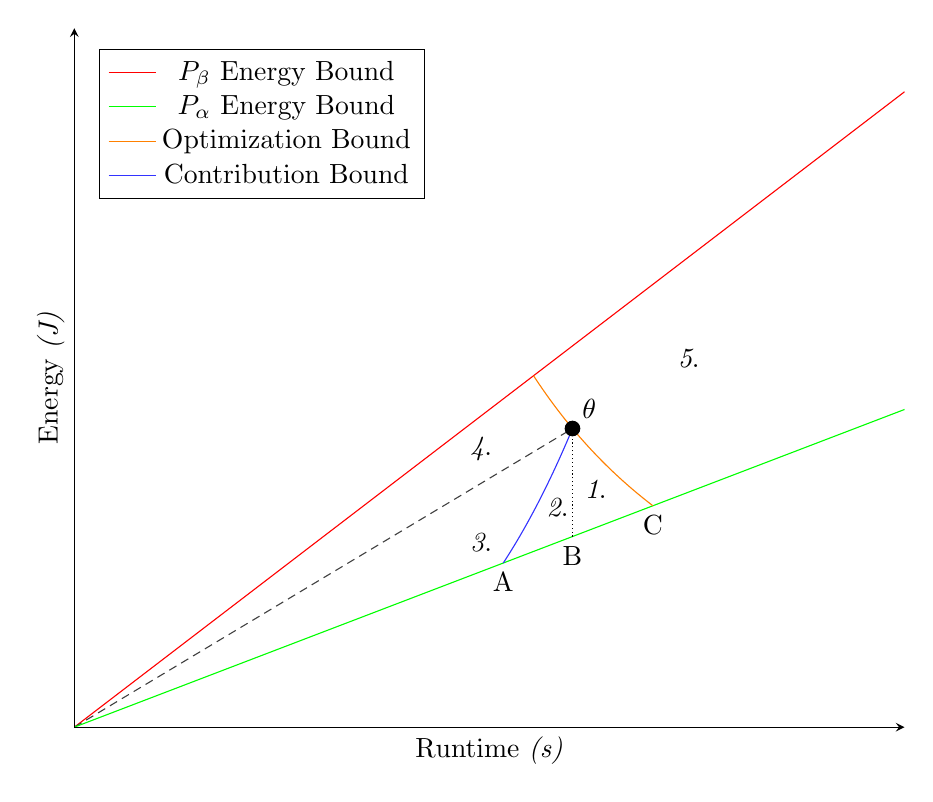
\begin{tikzpicture}
  \begin{axis}[ticks = none, 
    axis on top,
    axis x line=bottom,
    axis y line=left,
  	xlabel={Runtime \emph{(s)}},
    ylabel={Energy \emph{(J)}},    
    xmin=0, xmax=50,
    ymin=0, ymax=3300,
    width=\linewidth,
    legend style={legend pos=north west}
    ]

    %% Model Parameters %%
    \pgfmathsetmacro{\baselinepower}{30} % NOP code
    \pgfmathsetmacro{\rooflinepower}{60}
    \pgfmathsetmacro{\codepower}{47} 
    \pgfmathsetmacro{\codetime}{30}
    % Sadly, pgfplots sucks too much to calculate cube roots
    % These values are calculated with a ruby script in tools
    \pgfmathsetmacro{\anodex}{25.83028}
    \pgfmathsetmacro{\cnodex}{34.84283}
    \pgfmathsetmacro{\tnodex}{27.65477}

    \pgfmathsetmacro{\cnodey}{\cnodex * \baselinepower}
    \pgfmathsetmacro{\anodey}{\anodex * \baselinepower}
 
    %% Intermezzo Values %%
    \pgfmathsetmacro{\codeenergy}{\codepower * \codetime}
    \pgfmathsetmacro{\baselineenergy}{\baselinepower * \codetime}
    \pgfmathsetmacro{\rooflineenergy}{\rooflinepower * \codetime}
    \pgfmathsetmacro{\lowdisplayline}{(2 * \baselinepower + \codepower) / 3}
    \pgfmathsetmacro{\highdisplayline}{(1 * \rooflinepower + 1 * \codepower) / 2}

    % arguments: code power, code time, x - todo, apparently not supposed to do pgfmathparse
    \pgfmathdeclarefunction{metricbound}{3}{%
      \pgfmathparse{((#1 * #2^3) / #3^2)}%
    }
    \pgfmathdeclarefunction{definitionbound}{3}{%
      \pgfmathparse{((#1 / #2^3) * #3^4)}%
    }

    % BETA ROOFLINE BOUND
    \addplot[color=red, domain=\pgfkeysvalueof{/pgfplots/xmin}:\pgfkeysvalueof{/pgfplots/xmax}] {\rooflinepower * x};
    \addlegendentry{$P_{\beta}$ Energy Bound}

    %const power diagonal
    \addplot[color=darkgray, densely dashed, forget plot, %forget plot prevents legend entry
            domain=\pgfkeysvalueof{/pgfplots/xmin}:\codetime] {\codepower * x}; 

    % ALPHA BASELINE BOUND 
    \addplot[color=green, domain=\pgfkeysvalueof{/pgfplots/xmin}:\pgfkeysvalueof{/pgfplots/xmax}] {\baselinepower * x};
    \addlegendentry{$P_{\alpha}$ Energy Bound} 

    \addplot[color=orange, domain=\tnodex:\cnodex] { metricbound(\codepower, \codetime, x)};
    \addlegendentry{Optimization Bound}

    \addplot[color=blue!80, domain=\anodex:\codetime] { definitionbound(\codepower, \codetime, x)};
    \addlegendentry{Contribution Bound}

    % Constant Time, Energy Dashes
    %vertical
    \draw[densely dotted] ({axis cs:\codetime,\baselineenergy}) -- ({axis cs:\codetime,\codeenergy});

    \node[circle,fill,inner sep=2pt] at (axis cs:\codetime,\codeenergy) {};
    \node[above right] at (axis cs:\codetime,\codeenergy) {$\theta$};
    \pgfmathsetmacro{\oneycoord}{\lowdisplayline * 31.4}
    \node at (axis cs:31.4,\oneycoord) {\textit1.};
    \pgfmathsetmacro{\twoycoord}{\lowdisplayline * 29.1}
    \node at (axis cs:29.1,\twoycoord) {\textit2.};
    \pgfmathsetmacro{\threeycoord}{\lowdisplayline * 24.5}
    \node at (axis cs:24.5,\threeycoord) {\textit3.};
    \pgfmathsetmacro{\fourycoord}{\highdisplayline * 24.5}
    \node at (axis cs:24.5,\fourycoord) {\textit4.};
    \pgfmathsetmacro{\fiveycoord}{\codepower * 37}
    \node at (axis cs:37,\fiveycoord) {\textit5.};
    
    \node [below] at ({axis cs:\anodex, \anodey}) {A};
    \node [below] at ({axis cs:\codetime,\baselineenergy}) {B};
    \node [below] at ({axis cs:\cnodex, \cnodey}) {C};
    %\node [below, name intersections={of=metric bound and baseline}] at (intersection-1) {C};


 \end{axis}
\end{tikzpicture}

\caption{POSE for $ED^2P$}
\label{fig:technique}
\end{figure}

The POSE heuristic is based on the concept of a \emph{Feasible Performance Envelope}.
We construct this by plotting lines of gradient $P_{max}$ and $P_{min}$ in \autoref{fig:technique}.
These values represent the maximum and minimum rate of power consumption which can occur during normal operation of the target platform. By definition the $\langle Runtime, Energy\rangle$ costs incurred by running any given code $\theta$ on the target platform must be represented somewhere within this envelope.

To constrain our search space further we now consider the metric we wish to reduce.
For two logically equivalent codes $\theta$ and $\lambda$, the transformation ${\theta \to \lambda}$ is a valid optimization with respect to a cost metric $M$ if and only if ${M(\lambda) < M(\theta)}$.
We plot a curve passing through $\theta$ linking all points with ${M(\lambda) = M(\theta)}$.
By definition any optimized versions of $\theta$ can only exist below this optimization bound.

Naturally the equation for the optimization bound depends on the metric we are optimizing for.
\autoref{fig:technique} shows the optimization bound for $ED^2P$.
The general form of this bound for the $E^mD^n$ family of metrics is derived as follows:
\begin{align}
E^mD^n(\lambda) &= E^mD^n(\theta) \nonumber \\
\implies {E_\lambda}^m &= \frac{{E_\theta}^m{D_\theta}^n}{{D_\lambda}^n} \nonumber \\
\implies E_\lambda &= (\frac{{E_\theta}^m{D_\theta}^n}{{D_\lambda}^n})^\frac{1}{m}
\label{eq:optimization}
\end{align}

Our second bound considers what it means to optimize code for reduced power draw. 
An optimization $\theta \to \lambda$ with respect to metric $M$ is a power optimization if the change in power draw it delivers is responsible for the majority of the reduction in $M$. We plot a curve through $\theta$ linking all points with the same ratio of contributions to $M$ from both power and runtime factors as our original code. All valid power optimizations must lie below this contribution bound. 

Again the equation for the contribution bound depends on the metric chosen. 
\autoref{fig:technique} shows the bound for $ED^2P$ whilst the general form for $E^mD^n$ metrics is:
\begin{align}
\frac{{P_{\lambda}}^m}{{D_{\lambda}}^{m+n}} &= \frac{{P_{\theta}}^m}{{D_{\theta}}^{m+n}} \nonumber \\
\implies {P_{\lambda}}^m &= \frac{{P_{\theta}}^m}{{D_{\theta}}^{m+n}} \times {D_\lambda}^{m+n} \nonumber \\ 
\implies {E_{\lambda}}^m &= \frac{{P_{\theta}}^m}{{D_{\theta}}^{m+n}} \times {D_\lambda}^{m+n+1} \nonumber \\ 
\implies E_{\lambda} &= (\frac{{P_{\theta}}^m}{{D_{\theta}}^{m+n}} \times {D_\lambda}^{m+n+1})^{\frac{1}{m}} 
\end{align}

Intuitively it makes sense to use the most appropriate tools while searching for optimizations.  If an optimization yields dramatic reductions in runtime with only minor reductions in power consumption then it is reasonable to classify it as a runtime optimization and state that conventional time-based profilers and performance engineering tools are better suited to finding it. It is the contribution bound which enables our model to make this distinction.

The bounds described thus far allow us to identify the area of the Energy/Runtime plane in which optimized versions of a given code exist and to subdivide this space into runtime and power optimizations. The final component of POSE is the Optimization Limit, which subdivides the runtime optimized area of the feasible performance envelope into those optimizations which may be outperformed by power optimizations, and those which strictly dominate all possible power optimizations.

The optimization limit is based on \autoref{eq:optimization} and closely mirrors the the optimization bound.
This limit connects all points with the same value for $M$ as a hypothetical maximally power optimized version of $\theta$. 
All points below this limit have lower values for $M$, and therefore any optimizations in this area strictly dominate any possible power optimizations. 

Along with lines of constant time and power draw, these bounds allow us to subdivide \autoref{fig:technique} into the following labelled areas:
\begin{enumerate}
\item Power-only optimizations
\item Power-mostly optimizations
\item Time-mostly optimizations
\item Time-only optimizations
\item Performance Degradation
\end{enumerate}

Two key strengths of POSE are its simplicity and generality.
Only three measurements are required to build this plot; the system's baseline power draw, $P_{min}$, and the time and energy to solution for the code to be optimized, $D_\theta$ and $E_\theta$ respectively.
The precise value of $P_{max}$ can be ommitted when optimizing for power draw as we need not consider any values greater than our initial $P_\theta$.
We also need to consider which metric we are optimizing. \autoref{fig:technique} is based on $ED^2P$, whilst \autoref{fig:multimetric-technique} demonstrates how the POSE optimization area varies with metric choice.

POSE offers a wealth of information to performance engineers.
The difference in energy between $\theta$ and intercept $B$ places an upper limit on the absolute amount of energy which can be saved by power optimization alone.
The value $M(A) - M(\theta)$ bounds the amount of improvement in our metric we can expect to see from power optimization.
The difference in runtime between intersect $C$ and $\theta$ represents the maximum increase in runtime we could feasibly trade off to achieve a slower yet more energy efficient code.
Finally, the value $D(\theta) / D(A)$ represents the smallest speed-up which delivers more benefit than power optimization is capable of.

\begin{figure}
\centering
\begin{tikzpicture}
  \begin{axis}[ticks = none, 
    axis on top,
    axis x line=bottom,
    axis y line=left,
  	xlabel={Runtime \emph{(s)}},
    ylabel={Energy \emph{(J)}},    
    xmin=0, xmax=50,
    ymin=0, ymax=3300,
    width=\linewidth,
    legend style={legend pos=north west}
    ]

    %% Model Parameters %%
    \pgfmathsetmacro{\baselinepower}{30} % NOP code
    \pgfmathsetmacro{\rooflinepower}{60}
    \pgfmathsetmacro{\codepower}{47} 
    \pgfmathsetmacro{\codetime}{30}




    %% Intermezzo Values %%
    \pgfmathsetmacro{\codeenergy}{\codepower * \codetime}
    \pgfmathsetmacro{\baselineenergy}{\baselinepower * \codetime}
    \pgfmathsetmacro{\rooflineenergy}{\rooflinepower * \codetime}
    \pgfmathsetmacro{\lowdisplayline}{(2 * \baselinepower + \codepower) / 3}
    \pgfmathsetmacro{\highdisplayline}{(1 * \rooflinepower + 1 * \codepower) / 2}

    % arguments: code power, code time, x, n 
    \pgfmathdeclarefunction{metricbound}{4}{%
      \pgfmathparse{((#1 * #2^(#4 + 1)) / #3^#4)}%
    }
    \pgfmathdeclarefunction{definitionbound}{4}{%
      \pgfmathparse{((#1 / #2^(#4 + 1)) * #3^(#4 + 2))}%
    }
 
    % BETA ROOFLINE BOUND
    \addplot[color=red, domain=\pgfkeysvalueof{/pgfplots/xmin}:\pgfkeysvalueof{/pgfplots/xmax}] {\rooflinepower * x};
    \addlegendentry{$P_{\beta}$ Energy Bound}

    %const power diagonal
    \addplot[color=darkgray, densely dashed, name path=constpwr, forget plot, %forget plot prevents legend entry
            domain=\pgfkeysvalueof{/pgfplots/xmin}:\codetime] {\codepower * x}; 

    % ALPHA BASELINE BOUND 
    \addplot[color=green, name path=basebound, domain=\pgfkeysvalueof{/pgfplots/xmin}:\pgfkeysvalueof{/pgfplots/xmax}] {\baselinepower * x};
    \addlegendentry{$P_{\alpha}$ Energy Bound} 

    % Constant Time vertical dots
    %vertical
    \draw[densely dotted] ({axis cs:\codetime,\baselineenergy}) -- ({axis cs:\codetime,\codeenergy});

    % Sadly, pgfplots sucks too much to calculate cube roots
    % Domain values are calculated with a ruby script in tools

    %% Energy Area %%
    \addplot[name path=energy, draw=none, domain=19.14894:47, forget plot]{ min(definitionbound(\codepower, \codetime, x, 0),metricbound(\codepower, \codetime, x, 0))};
    \addplot[blue!6] fill between[of=energy and basebound];
    \addlegendentry{Energy}

    %% Energy Delay Product Area %% 
    \addplot[name path=edp, draw=none, domain=23.96806:37.54997, forget plot] { min(definitionbound(\codepower, \codetime, x, 1),metricbound(\codepower, \codetime, x, 1))};
    \addplot[blue!13] fill between[of=edp and basebound];
    \addlegendentry{$EDP$}

    %% Energy Delay Squared Product Area ##
    \addplot[name path=edtwop, draw=none, domain=25.83028:34.84283, forget plot] { min(definitionbound(\codepower, \codetime, x, 2),metricbound(\codepower, \codetime, x, 2))};
    \addplot[blue!21] fill between[of=edtwop and basebound];
    \addlegendentry{$ED^2P$}

    %% Energy Delay Cubed Product Area ##
    \addplot[name path=edthreep, draw=none, domain=26.81496:33.56336, forget plot] { min(definitionbound(\codepower, \codetime, x, 3),metricbound(\codepower, \codetime, x, 3))};
    \addplot[blue!35] fill between[of=edthreep and basebound];
    \addlegendentry{$ED^3P$}




     \node[circle,fill,inner sep=2pt] at (axis cs:\codetime,\codeenergy) {};
    \node[above right] at (axis cs:\codetime,\codeenergy) {$\theta$};
  \end{axis}
\end{tikzpicture}

\caption{Multiple Metric Code Optimization Spaces}
\label{fig:multimetric-technique}
\end{figure}
